%! TEX root = main.tex
\documentclass[main.tex]{subfiles}
\begin{document}
\section{Verfahren}
Im Jahr 1995 wurde nun ein dem SLA ähnliches Verfahren entwickelt, das Selective-Laser-Melting-Verfahren. Bei diesem wird statt dem Üblichen Photosensitiven UV-Kunstharz und einem UV-LCD feinstes Metallgranulat mit einem herkömmlichen Laser verwendet, welcher dieses in einem Pulverbett geanau zusammenschweißt. \parencite{3FAKTUR_1}
\begin{figure}[H]
\begin{center}
	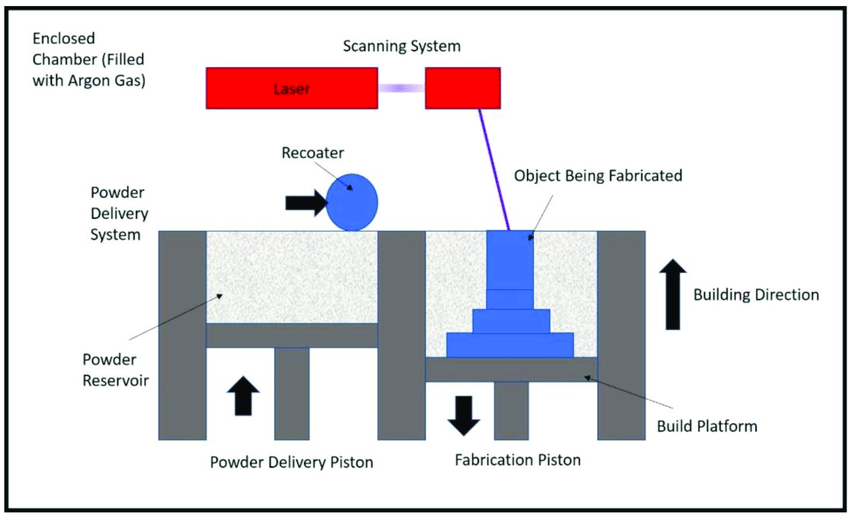
\includegraphics[width=.6\textwidth]{slm_diagram}
	\label{img:slm_diagram}
	\ccaption{Schematischer Aufbau einer SLM-Maschine}{\url{https://www.researchgate.net/publication/326891428/figure/fig1/AS:659597278855194@1534271654724/Schematic-diagram-of-the-selective-laser-melting-SLM-process.png}}
\end{center}
\end{figure}	
SLM ist ein Schichten-basierendes Verfahren. Das bedeutet, es trägt Schicht für Schicht auf
einer Bauplatform auf, welche sich danach nach unten bewegt um eine neue Schicht aufzutragen. 
Hinzukommt das SLM ein Pulverbett-Verfahren ist, was wiederrum bedeutet das eine neue perfekt ebene Schicht auf dem Baustück aufgetragen werden muss nach jedem Absenken der Platform.
Hierfür ist ein Wiederbeschichtungsroller vorhanden. Nach jeder Absenkung des Druckbettes wird über die Pulverlieferungsplatte die exakt gleiche Menge an Granulat nachgeliefert, welche dann vom Wiederbeschichtungsroller eben verteilt wird am Druckbett. 

Dieser Aufbau ist sehr simpel, jedoch sind eine große Menge an Variablen vorhanden, welche den Druck fehlschlagen lassen können.
\begin{itemize}
\item Fehlerhaftes Granulat
\item Falsche Stärke des Lasers
\item Falsche Schichtdicke
\item Zu wenig Pulver
	
\end{itemize}
Dennoch ist diese Vielseitigkeit der Grund warum SLM sich so großer Beliebtheit erfreut. Mit verschiendenen Temperaturen des Lasers lassen sich viele Materialien verarbeiten, die Schichtdicke bestimmt auch direkt die Druckdauer, da dickere Schichten zu weniger benötigten Schichten führen, was die Menge an Zeit die durch den Roller verbraucht wird verringert.
Eine solche Veränderung führt aber zu gröberen Teilen, welche danach nach-bearbeitet werden müssen (polieren, schleifen, drehen, etc.). 
\end{document}
